% ============================================================
% CHAPITRE 2 : ÉTUDE DE MARCHÉ
% ============================================================
\chapter{Étude de marché}
	\indent Dans un contexte où la logistique containerisée est au cœur des échanges commerciaux mondiaux, la question de la sécurité, de la traçabilité et de la transparence des opérations de transport devient un enjeu stratégique majeur. Les acteurs de la chaîne logistique (chargeurs, transporteurs, assureurs, clients finaux) sont confrontés à des risques multiples : vols, avaries, ruptures de chaîne du froid, litiges sur les responsabilités, etc. Face à ces défis, les solutions technologiques de suivi en temps réel, à l’instar des boîtes noires aéronautiques, apparaissent comme une réponse prometteuse pour offrir une visibilité totale et objective sur le parcours des conteneurs.

Le projet ARGOS vise précisément à concevoir et à réaliser une « boîte noire » intelligente pour conteneurs, capable d’enregistrer et de transmettre en continu des données critiques (position, température, chocs, ouvertures de porte, etc.) et de fournir une plateforme logicielle d’analyse et d’alerte. Cette étude de marché a pour objectif d’évaluer la pertinence commerciale, la demande potentielle et les attentes spécifiques des différents acteurs de la chaîne logistique, afin de guider la conception et le positionnement d’Argos.

Pour mener cette analyse, nous nous appuierons sur une enquête quantitative menée auprès d’un échantillon d’acteurs du secteur (clients, transporteurs, etc.), dont les résultats sont présentés dans ce chapitre. Nous identifierons également l’environnement concurrentiel, les forces et faiblesses du projet, et nous élaborerons une stratégie marketing complète (segmentation, ciblage, positionnement, marketing mix) permettant d’assurer le succès commercial d’Argos.

% ============================================================
% I. ANALYSE DE LA CLIENTÈLE
% ============================================================
\section{Analyse de la clientèle}

\indent L’analyse de la clientèle consiste à identifier les besoins, les attentes et les comportements des acteurs susceptibles d’utiliser la solution Argos. Elle s'appuie sur une enquête menée en ligne, couplée à des investigations sur le terrain auprès de professionnels du secteur. Les données ainsi collectées ont ensuite été traitées et analysées.
\subsubsection{Présentation de la méthode utilisée pour l'analyse}

Nous avons diffusé un questionnaire en ligne auprès d’un échantillon représentatif de la chaîne logistique : clients (chargeurs, entreprises de logistique), transporteurs, assureurs, et autres intervenants. Le questionnaire a été structuré en plusieurs sections couvrant les thèmes suivants :

\begin{itemize}
	\item \textbf{Profil du répondant} : rôle dans la chaîne, type d'activité, localisation géographique.
	\item \textbf{Problématiques rencontrées} : manque de transparence, litiges, vols, avaries, pertes financières.
	\item \textbf{Attentes vis-à-vis d'un dispositif de traçabilité} : spécifications techniques, fonctionnalités, modalités de suivi.
	\item \textbf{Préférences en matière de tarification et de service} : abonnement, budget, partage d'informations.
	\item \textbf{Confiance et perception des risques} : craintes liées au transport, intérêt pour une solution de type Argos.
\end{itemize}

L'enquête a été diffusée par courrier électronique et via des réseaux. Au total, 300 réponses ont été collectées. Le tableau \ref{tab:synthese-enquete} et le graphique associé récapitulent les caractéristiques de l'échantillon.

\begin{table}[H]
    \centering
    \caption{Synthèse de l’enquête (objectif de consolidation)}
    \label{tab:synthese-enquete}
    \begin{tabularx}{\textwidth}{@{}X>{\centering\arraybackslash}p{2.7cm}>{\centering\arraybackslash}p{2.2cm}@{}}
        \toprule
        \tableheadrow \thc{Éléments} & \thc{Taux cible} & \thc{Effectif} \\
        \midrule
        Questionnaires expédiés      & 100\,\% & 300 \\
        Questionnaires retournés     & 90\,\% & 270 \\
        Questionnaires non retournés & 10\,\% & 30 \\
        Questionnaires exploitables  & 83\,\% & 249 \\
        Questionnaires non exploitables & 7\,\% & 21 \\
        \bottomrule
    \end{tabularx}
    \tablesourcepromoteurs
\end{table}

\indent Le tableau récapitulatif de l’enquête met en évidence un taux de retour très satisfaisant de 90\,\% (270 questionnaires reçus sur 300 expédiés), témoignant de l'implication des parties prenantes ciblées. Parmi ces retours, une large majorité s'avère exploitable, représentant un taux de 83\,\% (249 questionnaires), tandis que la part des questionnaires non exploitables se limite à 7\,\% (21 questionnaires). Cette base de données finale offre ainsi un échantillon solide, rigoureux et statistiquement représentatif pour appuyer l'analyse et la consolidation des résultats du projet ARGOS.

\begin{figure}[H]
	\centering
	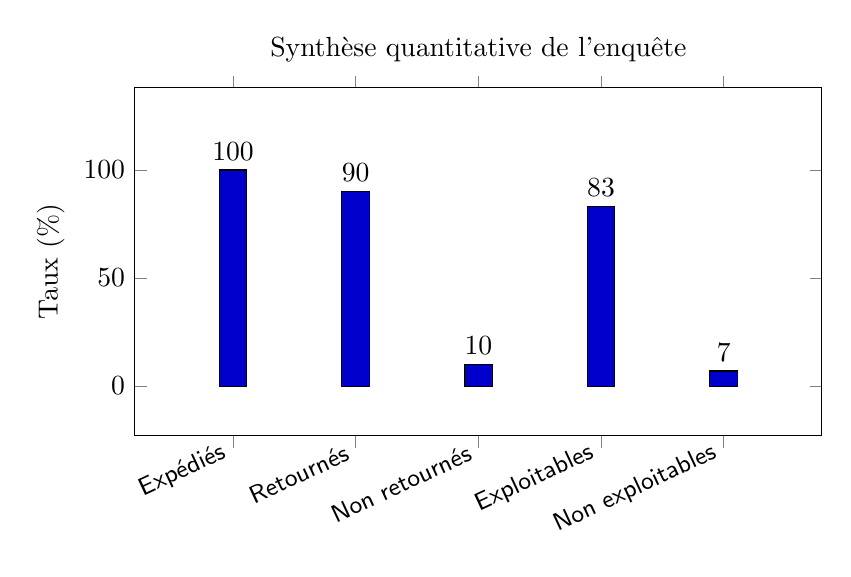
\begin{tikzpicture}
		\begin{axis}[
			title={Synthèse quantitative de l'enquête},
			ybar,
			enlargelimits=0.2,
			ylabel={Taux (\%)},
			symbolic x coords={Expédiés, Retournés, Non retournés, Exploitables, Non exploitables},
			xtick=data,
			x tick label style={rotate=25, anchor=east, font=\sffamily\small},
			nodes near coords,
			nodes near coords align={vertical},
			ymin=0, ymax=115,
			width=0.85\textwidth, height=6cm
		]
		\addplot[fill=blue!80!black] coordinates {
			(Expédiés,100)
			(Retournés,90)
			(Non retournés,10)
			(Exploitables,83)
			(Non exploitables,7)
		};
		\end{axis}
	\end{tikzpicture}
	\caption{Synthèse quantitative de l'enquête (Objectif de consolidation)}
	\label{fig-synthese-enquete-graphe}
    \tablesourcepromoteurs
\end{figure}

\subsubsection{Analyse des résultats}

Les résultats de l'enquête fournissent des indications claires sur les besoins, les attentes et les freins potentiels des acteurs de la logistique en matière de traçabilité des conteneurs.

\textbf{Question 1 : Quel est votre rôle dans la chaîne de distribution ?}

\begin{figure}[H]
	\centering
	\shorthandoff{:} % Désactive le double-point français pour éviter le bug
	\begin{tikzpicture}
		\pie[color={cyan!40, blue!80!black}]{86.8/Clients, 13.2/Transporteurs}
	\end{tikzpicture}
	\shorthandon{:} % Réactive le double-point français
	\caption{Répartition des répondants par rôle}
	\label{fig:roles}
    \tablesourcepromoteurs

\end{figure}

Les clients (industriels, particuliers) représentent 86,8\,\%, tandis que les transporteurs comptent 13,2\,\%. La très grande majorité des répondants sont donc des clients, ce qui reflète une demande forte et directe de la part des utilisateurs finaux de la chaîne logistique, qui sont en première ligne face aux aléas du transport. Les transporteurs, bien que moins nombreux, constituent un segment clé en tant qu’utilisateurs potentiels du dispositif embarqué.

\textbf{Question 2 : Existe-t-il une transparence dans la relation entre vous et les acteurs de logistique ?}

\begin{figure}[H]
	\centering
	\shorthandoff{:}
	\begin{tikzpicture}
		\pie[color={cyan!40, blue!80!black}]{34.1/Oui, 65.9/Non}
	\end{tikzpicture}
	\shorthandon{:}
	\caption{Perception de la transparence}
	\label{fig:transparence}
    \tablesourcepromoteurs

\end{figure}

Seulement 34,1\,\% des répondants estiment qu’il existe une transparence satisfaisante. Près de 65,9\,\% déclarent explicitement un manque de transparence. Ce constat est alarmant et souligne un besoin criant de solutions permettant de rendre les opérations plus lisibles et plus fiables.

\textbf{Question 3 : Considérez-vous qu’un équipement + un logiciel pourrait rendre la transparence plus claire ?}

\begin{figure}[H]
	\centering
	\shorthandoff{:}
	\begin{tikzpicture}
		\pie[color={cyan!40}]{100/Oui}
	\end{tikzpicture}
	\shorthandon{:}
	\caption{Intérêt pour une solution de traçabilité}
	\label{fig:interet}
    \tablesourcepromoteurs

\end{figure}

Une écrasante majorité (100\,\%) estime qu’un équipement de suivi associé à un logiciel pourrait améliorer la transparence. Ce résultat confirme l’opportunité commerciale d’Argos : les acteurs sont conscients que la technologie peut apporter une solution tangible à leurs difficultés de traçabilité et de confiance.

\textbf{Question 4 : Quelles spécifications techniques attendez-vous d’un tel dispositif ?}

Les réponses ouvertes ont été catégorisées ; les principales attentes sont résumées dans le tableau \ref{tab:spec-techniques}.

\begin{table}[H]
	\centering
	\caption{Spécifications techniques attendues}
	\label{tab:spec-techniques}
	\begin{tabularx}{\textwidth}{@{}X>{\centering\arraybackslash}p{3cm}@{}}
		\toprule
		\tableheadrow \thc{Spécification technique} & \thc{Citations (\%)} \\
		\midrule
		Résistance aux chocs / robustesse & 25,5\,\% \\
		Certification IP67 (étanchéité, poussière) & 13,5\,\% \\
		Autonomie longue durée (batterie) & 12,3\,\% \\
		Connectivité GSM / GPRS / satellite & 15,0\,\% \\
		Certifications ISO (qualité, sécurité) & 8,0\,\% \\
		Capteurs de température / humidité & 7,0\,\% \\
		Détection d’ouverture non autorisée (porte) & 18,7\,\% \\
		\bottomrule
	\end{tabularx}
    \tablesourcepromoteurs

\end{table}

\textbf{Question 5 : Quelles spécifications fonctionnelles attendez-vous ?}

\begin{table}[H]
	\centering
	\caption{Spécifications fonctionnelles attendues}
	\label{tab:spec-fonctionnelles}
	\begin{tabularx}{\textwidth}{@{}X>{\centering\arraybackslash}p{3cm}@{}}
		\toprule
		\tableheadrow \thc{Spécification fonctionnelle} & \thc{Pourcentage (\%)} \\
		\midrule
		Suivi en temps réel (position) & 39,5\,\% \\
		Alertes en cas d’anomalie (sortie de zone, choc) & 21,3\,\% \\
		Historique des trajets / tracé point par point & 10,2\,\% \\
		Accès auditeur / rapport d’incident & 10,8\,\% \\
		Partage de lien de suivi avec clients & 9,9\,\% \\
		Analyse des données (température, humidité) & 8,3\,\% \\
		\bottomrule
	\end{tabularx}
    \tablesourcepromoteurs

\end{table}

\textbf{Question 6 : Quelles sont vos principales craintes concernant le transport de marchandises ?}

\begin{figure}[H]
	\centering
	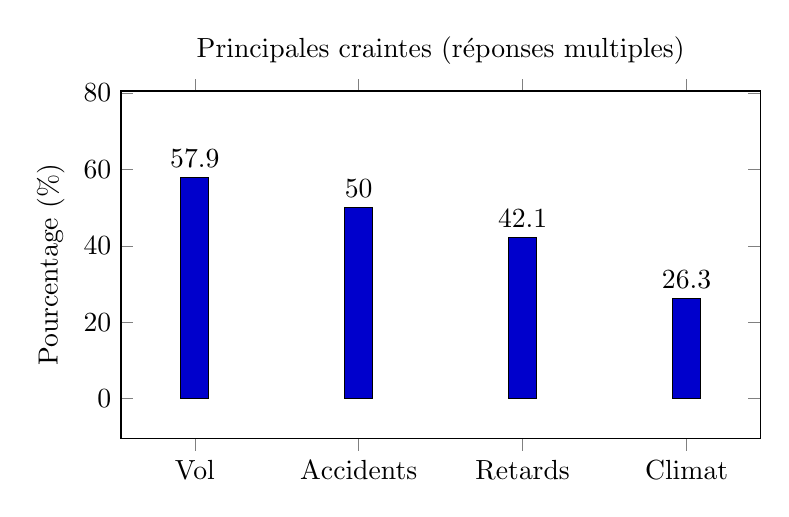
\begin{tikzpicture}
		\begin{axis}[
			title={Principales craintes (réponses multiples)},
			ybar,
			enlargelimits=0.15,
			ylabel={Pourcentage (\%)},
			symbolic x coords={Vol, Accidents, Retards, Climat},
			xtick=data,
			nodes near coords,
			nodes near coords align={vertical},
			ymin=0, ymax=70,
			width=0.8\textwidth, height=6cm
		]
		\addplot[fill=blue!80!black] coordinates {
			(Vol,57.9)
			(Accidents,50.0)
			(Retards,42.1)
			(Climat,26.3)
		};
		\end{axis}
	\end{tikzpicture}
	\caption{Principales craintes}
	\label{fig:craintes}
    \tablesourcepromoteurs

\end{figure}

Le vol arrive en tête avec 57,9\,\% des répondants, suivi des accidents avec 50,0\,\%, des retards avec 42,1\,\% et des risques climatiques avec 26,3\,\%. Comme il s’agit d’une question à réponses multiples, la somme des pourcentages peut dépasser 100\,\%. Ces résultats confirment que la sécurité physique des biens, la continuité du transport et la préservation de l’intégrité des marchandises sont au cœur des préoccupations. Argos, grâce à ses capteurs et à ses alertes, répond directement à ces risques.

\textbf{Question 7 : Quel pourcentage de la valeur de la marchandise seriez-vous prêt à investir pour garantir sa traçabilité ?}

\begin{figure}[H]
    \centering
    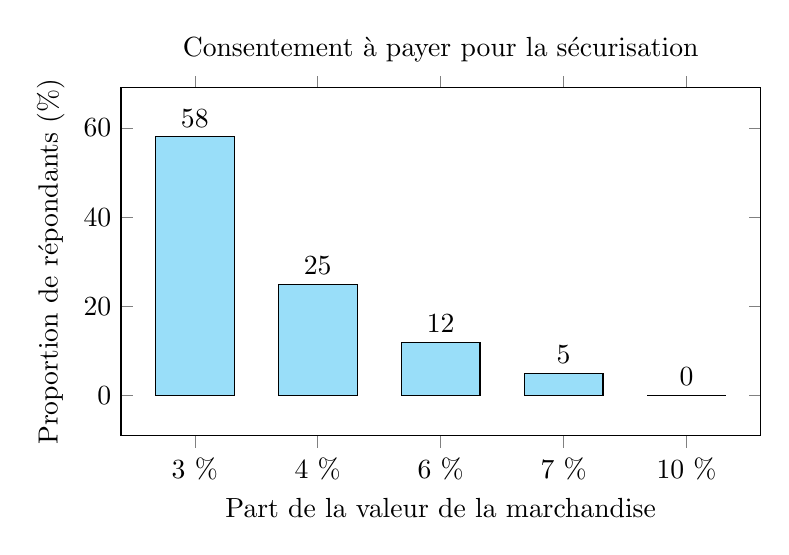
\begin{tikzpicture}
        \begin{axis}[
            title={Consentement à payer pour la sécurisation},
            ybar,
            enlargelimits=0.15,
            ylabel={Proportion de répondants (\%)},
            xlabel={Part de la valeur de la marchandise},
            symbolic x coords={3 \%, 4 \%, 6 \%, 7 \%, 10 \%},
            xtick=data,
            nodes near coords,
            nodes near coords align={vertical},
            ymin=0, ymax=60,
            width=0.8\textwidth, height=6cm,
            bar width=1cm
        ]
        \addplot[fill=cyan!40] coordinates {
            (3 \%,58)
            (4 \%,25)
            (6 \%,12)
            (7 \%,5)  % <--- CORRECTION ICI : "7 \%" au lieu de "7\%"
            (10 \%,0)
        };
        \end{axis}
    \end{tikzpicture}
    \caption{Consentement à payer pour la traçabilité des conteneurs}
    \label{fig:consentement_prix}
    \tablesourcepromoteurs
\end{figure}

Les résultats montrent que la majorité des acteurs (58\,\%) sont prêts à allouer jusqu'à 3\,\% de la valeur totale de leur marchandise pour s'assurer d'un suivi fiable et transparent. Seule une minorité est prête à investir 4\,\% ou 6\,\%, ce qui nous donne un excellent indicateur pour fixer la limite psychologique de notre tarification finale.

\textbf{Question 8 : Préférez-vous un abonnement annuel au logiciel ou un abonnement pour la durée du transit ?}

\begin{figure}[H]
	\centering
	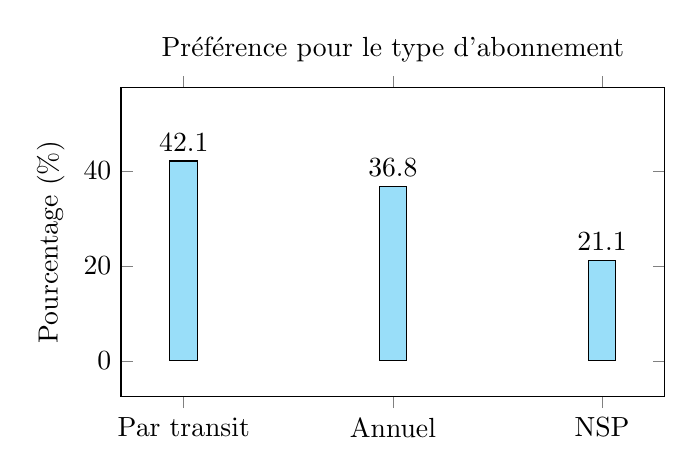
\begin{tikzpicture}
		\begin{axis}[
			title={Préférence pour le type d’abonnement},
			ybar,
			enlargelimits=0.15,
			ylabel={Pourcentage (\%)},
			symbolic x coords={Par transit, Annuel, NSP},
			xtick=data,
			nodes near coords,
			nodes near coords align={vertical},
			ymin=0, ymax=50,
			width=0.7\textwidth, height=5.5cm
		]
		\addplot[fill=cyan!40] coordinates {
			(Par transit,42.1)
			(Annuel,36.8)
			(NSP,21.1)
		};
		\end{axis}
	\end{tikzpicture}
	\caption{Préférence pour le type d’abonnement}
	\label{fig:abonnement}
    \tablesourcepromoteurs

\end{figure}

Les préférences sont relativement partagées : 42,1\,\% des répondants privilégient une formule par transit, 36,8\,\% préfèrent un abonnement annuel, et 21,1\,\% ne se prononcent pas (NSP). Cette répartition justifie le maintien de plusieurs formules adaptées aux utilisateurs réguliers et ponctuels.

\subsection{Synthèse globale des principaux renseignements}

Globalement, l’enquête met en évidence une adhésion élevée à la proposition de valeur d’Argos : 89,5\,\% estiment qu’un équipement associé à un logiciel peut améliorer la transparence et 73,7\,\% se déclarent intéressés par la surveillance à distance.

Les attentes se concentrent sur la robustesse, l’autonomie, la connectivité, la géolocalisation et les capteurs de condition. Les principales craintes exprimées sont le vol (57,9\,\%), les accidents (50,0\,\%), les retards (42,1\,\%) et les risques climatiques (26,3\,\%). Concernant les fonctions prioritaires, la géolocalisation recueille 39,5\,\% des citations, devant la détection d’ouverture (26,3\,\%), les alertes (23,7\,\%), la température (21,1\,\%) et la caméra (7,9\,\%).

Sur le plan commercial et financier, 42,1\,\% des répondants préfèrent une formule d'abonnement par transit et 36,8\,\% une formule annuelle. De plus, l'enquête révèle qu'une majorité d'acteurs (45\,\%) est disposée à investir jusqu'à 3\,\% de la valeur totale de leur marchandise pour en garantir la traçabilité. Argos a donc intérêt à proposer une tarification flexible (combinant achat du matériel avec abonnement SaaS ou location de dispositif avec services inclus), tout en veillant à ce que le coût global de la solution n'excède pas ce seuil psychologique de 3\,\%.

Ces tendances soutiennent la pertinence du projet pour orienter le prototype et la stratégie commerciale. Leur généralisation au marché devra toutefois être confirmée par l’échantillon élargi prévu dans le tableau de synthèse et par des entretiens ciblés avec les décideurs portuaires, maritimes, logistiques et assurantiels.
% ============================================================
% II. ANALYSE DE LA CONCURRENCE
% ============================================================
\section{Analyse de la concurrence}

L'environnement concurrentiel du projet Argos regroupe un ensemble de solutions de suivi et de traçabilité de conteneurs, allant des trackers GPS aux systèmes IoT embarqués, en passant par les plateformes logistiques et les services d'assurance spécialisés. 

Afin d'évaluer la position stratégique du projet sur le marché, l'étude concurrentielle s'articule autour de deux catégories distinctes d'acteurs, synthétisées dans les sections et tableaux ci-après.

\subsubsection{Concurrents directs} 

\indent Cette première catégorie regroupe les entreprises proposant des solutions matérielles et logicielles directement concurrentes, dotées de fonctionnalités similaires en matière de géolocalisation, de télémétrie et d'alertes en temps réel. Le Tableau \ref{tab:concurrents-directs} met en lumière les forces et les faiblesses de ces acteurs de référence sur le marché international.


\begin{table}[H]
    \centering
    \caption{Analyse des concurrents directs}
    \label{tab:concurrents-directs}
    \begin{tabularx}{\textwidth}{@{}>{\raggedright\arraybackslash}p{0.23\textwidth}XX@{}}
        \toprule
        \tableheadrow \thc{Concurrent} & \thc{Forces} & \thc{Faiblesses} \\
        \midrule
        \textbf{Tive} & Technologie avancée, plateforme web complète, notoriété internationale. & Coût élevé, abonnement onéreux, inadapté aux réalités locales. \\
        \textbf{Roambee} & Capteurs multiples, analyse prédictive, intégration ERP. & Prix élevé, dépendance au réseau cellulaire, complexité. \\
        \textbf{Nexxiot} & Approche cargo-intelligence, partenariats assureurs. & Solution industrielle, coût d'entrée élevé. \\
        \bottomrule
    \end{tabularx}
    \tablesourcepromoteurs
\end{table}

\subsubsection{Concurrents indirects} 

\indent L'analyse se poursuit avec les solutions alternatives qui répondent partiellement aux besoins de traçabilité du fret, tout en présentant des limites fonctionnelles majeures face à l'approche intégrée d'Argos. Les caractéristiques de ces offres sont détaillées dans le Tableau \ref{tab:concurrents-indirects}.

\begin{table}[H]
    \centering
    \caption{Analyse des concurrents indirects}
    \label{tab:concurrents-indirects}
    \begin{tabularx}{\textwidth}{@{}>{\raggedright\arraybackslash}p{0.23\textwidth}XX@{}}
        \toprule
        \tableheadrow \thc{Concurrent} & \thc{Forces} & \thc{Faiblesses} \\
        \midrule
        \textbf{Trackers GPS standards} & Faible coût, autonomie longue. & Pas de capteurs environnementaux, données brutes. \\
        \textbf{Solutions d'assurance} & Intégration dans les polices, réduction de prime. & Limité au suivi de position, manque de flexibilité. \\
        \bottomrule
    \end{tabularx}
    \tablesourcepromoteurs
\end{table}
\subsection{Analyse SWOT}
L’analyse SWOT (Forces, Faiblesses, Opportunités, Menaces) permet de synthétiser les atouts et les défis du projet Argos. Afin de positionner stratégiquement la solution face aux réalités du marché et aux exigences technologiques, le Tableau \ref{tab:swot} dresse un panorama croisé de l'environnement interne et externe du projet.
\begin{table}[H]
    \caption{Analyse SWOT d’Argos}
    \label{tab:swot}
    \renewcommand{\arraystretch}{1.3} % Donne un peu plus d'espace aux lignes
    \begin{tabularx}{\textwidth}{@{}XX@{}}
        \toprule
        \tableheadrow \thc{Forces} & \thc{Faiblesses} \\
        \midrule
        \textbullet~ Solution complète (matériel + logiciel) adaptée aux besoins des acteurs locaux et internationaux.
        
        \textbullet~ Maîtrise des nouvelles technologies de géolocalisation, IoT, capteurs et communication de données.
        
        \textbullet~ Conception orientée vers le respect des exigences applicables de l’OMI et des standards internationaux de sécurité des conteneurs \cite{omi2026,iso2018}.
        
        \textbullet~ Production de preuves numériques horodatées et sécurisées, conçues pour être difficilement altérables lors des litiges ou pertes.
        & 
        \textbullet~ Coût initial élevé (matériel, certification, cloud et déploiement).
        
        \textbullet~ Dépendance à la couverture réseau dans certaines zones.
        
        \textbullet~ Sensibilisation du marché nécessaire pour expliquer les bénéfices.
        
        \textbullet~ Besoins d’homologation et de standardisation avant un déploiement à grande échelle. \\
        
        \midrule
        \tableheadrow \thc{Opportunités} & \thc{Menaces} \\
        \midrule
        \textbullet~ Croissance du commerce mondial et du transport conteneurisé.
        
        \textbullet~ Demande accrue de traçabilité et de transparence de la part des clients finaux.
        
        \textbullet~ Renforcement des exigences OMI et de la numérisation maritime : évolution susceptible de favoriser à terme l’adoption des conteneurs intelligents. À ce jour, aucune obligation générale de l’OMI n’impose les smart containers \cite{imo_web,wsc2025}.
        
        \textbullet~ Potentiel d’innovation dans l’analyse prédictive (IA) et la blockchain pour la traçabilité.
        & 
        \textbullet~ Arrivée de nouveaux concurrents avec des technologies avancées.
        
        \textbullet~ Brouillage du GPS et cyberattaques pouvant perturber la disponibilité ou l’intégrité des données.
        
        \textbullet~ Détournement ou manipulation physique du dispositif et du conteneur.
        
        \textbullet~ Résistance au changement de certains acteurs traditionnels. \\
        \bottomrule
    \end{tabularx}
    \tablesourcepromoteurs
\end{table}

\noindent \textbf{Bilan de l'analyse stratégique~:} 
Il ressort de cette matrice que le projet ARGOS dispose d'une réelle valeur ajoutée technologique et d'un positionnement opportun face aux mutations de la supply chain. Si les faiblesses et menaces identifiées, telles que les coûts initiaux, les barrières d'homologation ou les risques cyber, nécessitent une gestion rigoureuse des risques et une stratégie d'accompagnement du marché, les opportunités de croissance et l'alignement avec les exigences normatives confirment la viabilité et la pertinence à long terme de la solution.
% ============================================================
% III. STRATÉGIE MARKETING ET MARKETING-MIX (4P)
% ============================================================
\section{Élaboration de la stratégie marketing}
La stratégie marketing d’Argos marque une rupture avec les modèles traditionnels : nous ne vendons pas de matériel. Argos se positionne comme un fournisseur de services de traçabilité (Traçabilité as a Service - TaaS). L'objectif est d'équiper massivement les flottes de conteneurs pour sécuriser le fret à forte valeur ajoutée.
\subsection{Segmentation du marché}
Afin d'adresser efficacement les spécificités de la chaîne logistique, le marché potentiel d'Argos a été segmenté selon les critères structurants suivants :
\begin{itemize}[label=\textcolor{argosblue}{\textbf{>}}]
    \item \textbf{Type d’acteur}~: Distinction entre les propriétaires de conteneurs (compagnies maritimes, loueurs) qui gèrent les actifs physiques et les utilisateurs finaux (chargeurs, industriels, exportateurs) qui en supportent les risques opérationnels.
    \item \textbf{Nature de la marchandise}~: Segmentation par niveau de criticité, ciblant prioritairement les marchandises à forte valeur ajoutée ou sensibles (produits pharmaceutiques, équipements électroniques, denrées périssables), pour lesquelles le coût de la sécurité demeure marginal au regard de la valeur du fret.
    \item \textbf{Critères géographiques}~: Cartographie des hubs logistiques majeurs et des corridors de transit terrestre présentant des zones de vulnérabilité élevée (risques de vols, de retards ou de dégradations structurelles)\cite{logcluster}.
\end{itemize}

\subsection{Ciblage du marché et modèle économique}

Le ciblage d'Argos repose sur une synergie vertueuse entre les détenteurs d'actifs logistiques et les expéditeurs de marchandises.

\subsubsection{Cible principale (Les partenaires d'équipement)}
L'engagement de ces acteurs clés s'articule autour des dimensions suivantes :
\begin{itemize}[label=\textcolor{argosblue}{\textbf{>}}]
    \item \textbf{Acteurs}~: Compagnies maritimes, armateurs, et agences propriétaires de flottes de conteneurs.
    \item \textbf{Besoins}~: Moderniser leur parc vers le concept de \textit{smart containers} sans supporter d'investissement en capital lourd (Capex), fidéliser leur clientèle par un service à forte valeur ajoutée, et générer de nouveaux flux de revenus récurrents.
    \item \textbf{Notre offre (Le partenariat)}~: Nous leur fournissons et installons le dispositif Argos \textbf{gratuitement}. En contrepartie, ces partenaires intègrent notre solution directement au cœur de leur offre logistique.
\end{itemize}

\subsubsection{Cible secondaire}
La réponse aux exigences de ces utilisateurs finaux se structure de la manière suivante :
\begin{itemize}[label=\textcolor{argosblue}{\textbf{>}}]
    \item \textbf{Acteurs}~: Chargeurs, importateurs/exportateurs, et industriels.
    \item \textbf{Besoins}~: Garantie absolue d’intégrité de la cargaison, visibilité logistique de bout en bout et production de preuves juridiques incontestables en cas de litige ou d’avarie.
    \item \textbf{Notre offre (Le service)}~: Ils souscrivent au service de suivi Argos lors de l’expédition afin d'assurer l’intégrité de leur fret et d'accélérer les procédures d'indemnisation.
\end{itemize}

\subsubsection{Le modèle de revenus}
Contrairement aux schémas d'acquisition classiques, Argos adopte un modèle de tarification à l'usage adossé à la valeur réelle de la marchandise transportée :
\begin{itemize}[label=\textcolor{argosblue}{\textbf{>}}]
    \item \textbf{Facturation client}~: À chaque expédition, le client s’acquitte de frais de sécurisation fixés à \textbf{3\,\% de la valeur déclarée de la marchandise}.
    \item \textbf{Rétrocession partenaire (40\,\%)}~: Sur cette redevance, \textbf{40\,\% sont reversés directement à l'agence} propriétaire du conteneur. Ce reversement compense l'hébergement physique du boîtier, couvre les frais de maintenance de premier niveau et absorbe les aléas opérationnels.
    \item \textbf{Revenu Argos (60\,\%)}~: Les \textbf{60\,\% restants} constituent le chiffre d’affaires net d’Argos, destiné à l’amortissement du matériel, aux coûts du cloud, à la connectivité hybride et à l'exploitation de la plateforme logicielle SaaS.
\end{itemize}

\subsection{Marketing-Mix (4P)}

Afin de traduire la stratégie de positionnement d'ARGOS en actions opérationnelles sur le marché, nous avons structuré notre offre autour du modèle du Marketing-Mix (les 4P). Cette démarche permet de décliner concrètement notre approche de « Traçabilité as a Service » (TaaS) à travers quatre axes fondamentaux : la définition exacte du service apporté (Produit), notre modèle tarifaire innovant (Prix), nos canaux de déploiement (Place) et nos actions pour convaincre les acteurs logistiques (Promotion)

\subsubsection{Politique de produit (service)}
L'offre d'Argos ne se résume pas à un simple boîtier matériel, mais constitue une \textbf{solution globale de sécurisation et de télémétrie} structurée autour des prestations suivantes :
\begin{itemize}[label=\textcolor{argosblue}{\textbf{>}}]
    \item Mise à disposition et installation du matériel embarqué (IoT) sur les parcs de conteneurs partenaires.
    \item Accès unifié à une plateforme SaaS en temps réel offrant la géolocalisation continue, le suivi des chocs, de l'humidité, de la température et des alertes d'ouverture.
    \item Édition automatisée de preuves numériques horodatées, sécurisées et juridiquement opposables en cas de litige commercial.
    \item Gestion technique simplifiée via des mises à jour logicielles à distance (OTA) et une maintenance de proximité déléguée au réseau partenaire.
\end{itemize}

\subsubsection{Politique de prix}
La stratégie tarifaire repose sur un modèle disruptif aligné sur le risque et la valeur ajoutée transportée :
\begin{itemize}[label=\textcolor{argosblue}{\textbf{>}}]
    \item \textbf{Prix du matériel}~: 0 FCFA. Le dispositif est déployé sous forme de mise à disposition gratuite.
    \item \textbf{Tarification du service}~: \textbf{3\,\% de la valeur de la marchandise} par trajet effectué.
    \item \textbf{Partage des revenus (Revenue Share)}~: Répartition rigoureuse de 40\,\% au profit du transporteur (frais de gestion et maintenance) et de 60\,\% pour Argos (exploitation SaaS, valorisation des données et rentabilité).
\end{itemize}
\textit{Justification économique}~: Un industriel acheminant pour 100\,000 fcfa de composants électroniques ou de denrées sensibles légitime instantanément un investissement de 3\,000 fcfa pour s'immuniser contre les pertes totales et garantir l'intégrité de son fret.

\subsubsection{Politique de place (distribution)}
L'architecture de distribution combine des accords institutionnels et un canal d'intégration opérationnel :
\begin{itemize}[label=\textcolor{argosblue}{\textbf{>}}]
    \item \textbf{Intégration directe (B2B)}~: La pénétration du marché s'effectue par la signature d'accords-cadres stratégiques conclus directement avec les compagnies maritimes, les armateurs et les gestionnaires de parcs de conteneurs.
    \item \textbf{Canal indirect pour l'utilisateur}~: L'accès au service pour le client final se fait de manière fluide au guichet de son transitaire ou de sa compagnie maritime au moment de la réservation du fret, en sélectionnant l’option de service « Fret Sécurisé ».
\end{itemize}

\subsubsection{Politique de promotion (communication)}
L'effort de communication vise à évangéliser ce nouveau paradigme B2B2C selon les axes opérationnels suivants :
\begin{itemize}[label=\textcolor{argosblue}{\textbf{>}}]
    \item \textbf{Vers les transporteurs (Cible B2B directe)}~: Déploiement d'une prospection active, démonstrations physiques sur les terminaux portuaires, participation active aux salons professionnels de la logistique et mise en avant de l'argument financier.
    \item \textbf{Vers les clients finaux (Cible B2B/B2C)}~: Déploiement d'une stratégie de marketing digital ciblée (campagnes sur les réseaux professionnels et moteurs de recherche axées sur la sécurité logistique) et publication de livres blancs sectoriels dédiés à la réduction des litiges.
\end{itemize}
\begin{longtable}{@{}>{\raggedright\arraybackslash}p{2.5cm} >{\raggedright\arraybackslash}p{6.1cm} >{\centering\arraybackslash}p{1.2cm} >{\centering\arraybackslash}p{2.1cm} >{\centering\arraybackslash}p{2.1cm}@{}}
\caption{Budget prévisionnel de communication} \label{tab:budget_communication} \\
\toprule
\textbf{Supports} & \textbf{Observations} & \textbf{Qté} & \textbf{P.U. (FCFA)} & \textbf{Total (FCFA)} \\
\midrule
\endfirsthead
\multicolumn{5}{c}{\tablename\ \thetable{} -- Suite de la page précédente} \\
\toprule
\textbf{Supports} & \textbf{Observations} & \textbf{Qté} & \textbf{P.U. (FCFA)} & \textbf{Total (FCFA)} \\
\midrule
\endhead
\midrule
\multicolumn{5}{r}{\textit{...}} \\
\endfoot
\bottomrule
\multicolumn{5}{l}{\textit{Source : Les Promoteurs 2025-2026 -- Budget total : 600 000 FCFA}} \\
\endlastfoot
\multicolumn{5}{@{}l@{}}{\textbf{MÉDIAS}} \\
Affichage extérieur & Visibilité dans les zones portuaires et professionnelles & 1 & 100 000 & 100 000 \\
Internet / médias numériques & Site web, LinkedIn, YouTube, Google Ads / LinkedIn Ads et contenus de démonstration & 1 & 250 000 & 250 000 \\
\midrule
\multicolumn{5}{@{}l@{}}{\textbf{HORS MÉDIA}} \\
Salons et conférences & Participation aux événements professionnels du secteur maritime et logistique & 1 & 150 000 & 150 000 \\
Flyers, brochures et goodies & Supports physiques de présentation et de promotion d'ARGOS & 1 & 50 000 & 50 000 \\
Démonstrations / webinaires & Présentation directe du boîtier et démonstrations de la solution & 1 & 50 000 & 50 000 \\
\midrule
\textbf{TOTAL GENERAL} & & & & \textbf{600 000} \\
\end{longtable}

\indent \textbf{Bilan du budget de communication~:} 
L’analyse de la ventilation financière de la campagne met en lumière une orientation résolument numérique et ciblée. Avec une enveloppe globale de 600\,000 FCFA, l'effort promotionnel priorise les médias digitaux et les réseaux professionnels (représentant 250\,000 FCFA, soit plus de 41\,\% du budget), garantissant une visibilité directe auprès des décideurs logistiques et des chargeurs. L'allocation complémentaire vers les salons professionnels (150\,000 FCFA) et l'affichage stratégique en zone portuaire permet d'ancrer la solution dans l'écosystème physique du transport, assurant ainsi un équilibre optimal entre prospection de terrain et notoriété numérique.

% ============================================================
% V. STRATÉGIE DE MARKETING DIGITAL
% ============================================================

\subsection{Stratégie de positionnement}

La stratégie d’Argos s'articule autour d'un dispositif multicanal conçu pour rassurer les grands comptes, asseoir la crédibilité technique de la solution et dynamiser l'acquisition B2B :
\begin{itemize}[label=\textcolor{argosblue}{\textbf{>}}]
    \item \textbf{Présence web institutionnelle}~: Déploiement d’un portail vitrine centralisant les études de cas sectorielles, la documentation sur l'architecture matérielle et logicielle, ainsi que les garanties relatives à la sécurité et à l'intégrité des données transmises.
    
    \item \textbf{Réseau professionnel B2B (LinkedIn)}~: Animation d’une page active axée sur le partage d'expertises (articles techniques sur la gestion des risques liés aux avaries maritimes, la réduction des litiges sur les corridors et les avantages économiques du modèle de \textit{Revenue Share} pour les armateurs).
    
    \item \textbf{Inbound Marketing et conversion}~: Mise en place d’outils interactifs, tels que des simulateurs de retour sur investissement en ligne, permettant aux chargeurs de mesurer instantanément les gains économiques générés par la sécurisation de leur fret au regard de la redevance de service.
    
    \item \textbf{Séminaires et démonstrations sectorielles}~: Organisation d'ateliers professionnels et de présentations physiques ciblées (roadshows) auprès des décideurs portuaires, maritimes et douaniers, leur permettant de tester concrètement la robustesse du dispositif embarqué et la réactivité de la plateforme d'alerte.
    
    \item \textbf{Formation et accompagnement des partenaires}~: Mise en place de modules de capacitation technique et commerciale destinés au personnel de nos partenaires (compagnies maritimes, transitaires, etc). Cet accompagnement garantit une installation fluide des boîtiers sur les conteneurs (onboarding) et assure que leurs équipes de vente maîtrisent parfaitement les arguments pour proposer des meilleurs option aux clients finaux.
\end{itemize}

% ============================================================
% CONCLUSION DU CHAPITRE
% ============================================================
\indent L’étude de marché et la stratégie qui en découle confirment le positionnement innovant d'Argos. En abandonnant la vente de matériel au profit d'un modèle de service indexé sur la valeur de la marchandise (3\,\%), Argos lève la barrière à l'entrée du coût d'équipement pour les transporteurs. Ce modèle tripartite gagnant-gagnant garantit une sécurité maximale aux chargeurs, de nouveaux revenus pour les propriétaires de conteneurs, et une croissance scalable pour Argos. La validation de ce modèle sera éprouvée lors des phases pilotes avec nos premiers partenaires logistiques, abordées dans les études techniques de ce rapport.
